\documentclass[11pt]{article}
\usepackage[margin=1in]{geometry}
\usepackage{mathptmx}
\usepackage[T1]{fontenc}
\usepackage{microtype}
\usepackage{amsmath, amssymb}
\usepackage{tabularx}
\usepackage{graphicx}
\usepackage{booktabs}
\usepackage{array}
\usepackage{xcolor}
\usepackage{listings}
\usepackage{enumitem}
\usepackage[hypcap=false]{caption}
\usepackage[hidelinks]{hyperref}

% --------------------------------------------------------------------------------------------
% Open, Readable Typography & Spacing
% --------------------------------------------------------------------------------------------
\linespread{1.08}
\setlength{\parskip}{0.45em}
\setlength{\parindent}{0pt}
\renewcommand{\arraystretch}{1.28}

\definecolor{codebg}{rgb}{0.975, 0.978, 0.985}
\definecolor{codecomment}{rgb}{0.22, 0.48, 0.32}
\definecolor{codekeyword}{rgb}{0.05, 0.22, 0.65}
\definecolor{codenumbers}{rgb}{0.52, 0.52, 0.52}
\definecolor{codestring}{rgb}{0.68, 0.12, 0.12}
\definecolor{accentblue}{rgb}{0.10, 0.32, 0.55}

\lstdefinestyle{gostyle}{
    backgroundcolor=\color{codebg},
    commentstyle=\color{codecomment}\itshape,
    keywordstyle=\color{codekeyword}\bfseries,
    stringstyle=\color{codestring},
    numberstyle=\tiny\color{codenumbers},
    basicstyle=\ttfamily\footnotesize,
    breaklines=true,
    numbers=left,
    numbersep=6pt,
    frame=single,
    rulecolor=\color{black!18},
    tabsize=4,
    xleftmargin=1.2em,
    framexleftmargin=1.2em,
    aboveskip=8pt,
    belowskip=8pt,
    morekeywords={package,import,func,type,struct,interface,var,const,return,if,else,for,range,go,select,case,default,switch,defer,chan,make,len,cap,copy,nil,true,false,int,int64,uint64,bool,string,float64,time,context}
}

\lstdefinestyle{logstyle}{
    backgroundcolor=\color{codebg},
    basicstyle=\ttfamily\footnotesize,
    breaklines=true,
    numbers=none,
    frame=single,
    rulecolor=\color{black!18},
    xleftmargin=0.6em,
    framexleftmargin=0.6em,
    aboveskip=6pt,
    belowskip=8pt
}
\lstset{style=gostyle}

\setlist[itemize]{leftmargin=1.4em, itemsep=0.28em, topsep=0.25em}
\setlist[enumerate]{leftmargin=1.5em, itemsep=0.32em, topsep=0.25em}
\captionsetup{font=small, labelfont=bf, skip=6pt}

\newcommand{\partheader}[1]{%
    \vspace{1.0em}%
    {\noindent\fontsize{13.5}{16}\selectfont\textbf{\color{accentblue}#1}\par}%
    \vspace{0.2em}\hrule\vspace{0.7em}%
}
\newcommand{\subhead}[1]{\vspace{0.6em}\noindent\textbf{\large #1}\par\vspace{0.25em}}

\begin{document}
\emergencystretch=1.8em

% ============================================================================================
% TITLE PAGE
% ============================================================================================
\begin{titlepage}
\begin{center}
    \vspace*{0.6cm}
    
\includegraphics[width=0.26\textwidth]{VNIT_logo.jpg}\\[1.0cm]

    {\large \textbf{Group Members}}\\[0.3cm]
    \begin{tabular}{l c l}
        Student 1: Gaurav Acharya & --- & [MT26MCS024] \\
        Student 2: Sandeep & --- & [MT26MCS032]
    \end{tabular}

    \vspace{0.9cm}

    {\large \textbf{Course \& Faculty Guide}}\\[0.25cm]
    CSP502 Software Lab-I --- M.Tech.\ CSE W26\\
    Visvesvaraya National Institute of Technology (VNIT), Nagpur\\
    Faculty Guide: Dr.\ A.\ S.\ Mokhade

    \vspace{0.9cm}

    {\large \textbf{Practical Title}}\\[0.25cm]
    {\Large \textbf{Practical 8: From Resilience to Reliability --- Testing and Observing a Concurrent Service in Go}}

    \vspace{3cm}

    \small
    \begin{tabular}{ll}
        \toprule
        \textbf{Environment} & \textbf{Specification} \\
        \midrule
        Go Toolchain & \texttt{go1.27.1-X:nodwarf5 linux/amd64} \\
        Machine & 12th Gen Intel Core i7-12650H (10C/16T), Linux \\
        Workload & $N = 1{,}200$ reqs/run, $W = 8$ workers, seeds $\{101, 202, 303\}$ \\
        \bottomrule
    \end{tabular}
\end{center}
\end{titlepage}

% ============================================================================================
% PART A
% ============================================================================================
\partheader{Part A --- Tutorial Analysis and Pre-Coding Test Plan}

\textbf{Design Record:} Frozen \texttt{2026-11-18T14:15:00+05:30} (\path{docs/partA_design_record.md}).\\
\textbf{Go References Cited:} \textit{Add a test} (Write/Run/Failing test), \textit{Race Detector} (Usage, Report Format, Overheads), \texttt{context} (\texttt{WithCancel}, \texttt{WithTimeout}, \texttt{Done}), and \textit{Pipelines} (Stopping short, Explicit cancellation).

\subhead{A1. Claim Classification}
\begin{table}[htbp]
\centering
\caption{Classification of Reliability and Testing Claims.}
\footnotesize
\begin{tabularx}{\textwidth}{@{} >{\raggedright\arraybackslash}p{4.3cm} >{\raggedright\arraybackslash}p{2.1cm} >{\raggedright\arraybackslash}X @{}}
\toprule
\textbf{Claim} & \textbf{Classification} & \textbf{Reasoning} \\
\midrule
1. One successful run proves no request can be lost. & \textbf{Unjustified} & Concurrent schedules vary across runs; one interleaving cannot rule out races, drops, or shutdown losses. \\
2. A \texttt{-race} pass proves no deadlock is possible. & \textbf{Unjustified} & \texttt{-race} detects unsynchronized memory writes on executed paths; deadlocks are liveness failures that happen in race-free code. \\
3. Retrying is harmless if the result is recorded once. & \textbf{Conditionally Justified} & Safe only when the retried work has no duplicate external side effects and retries use bounded backoff/budgets. \\
4. Clean shutdown may reject new requests while finishing accepted ones. & \textbf{Justified} & Closing intake makes the backlog finite so accepted requests can drain within a bounded grace period. \\
5. Low mean latency guarantees good tail latency. & \textbf{Unjustified} & Means hide heavy tails; 5\% slow requests can push p95/p99 past 500\,ms while keeping mean near 30\,ms. \\
\bottomrule
\end{tabularx}
\end{table}

\subhead{A2. Testable Invariants, Boundaries, and Predictions}
\begin{itemize}
    \item \textbf{I1 (Accounting Conservation):} $N_{\text{generated}} = N_{\text{success}} + N_{\text{failure}} + N_{\text{timeout}} + N_{\text{cancelled}} + N_{\text{rejected}}$, with $N_{\text{missing}} = 0$.
    \item \textbf{I2 (Unique Terminal Outcome):} Each unique \texttt{RequestID} commits exactly one immutable terminal outcome ($N_{\text{dup}} = 0$).
    \item \textbf{I3 (Lifecycle Ordering):} Event sequence numbers obey \texttt{generated} $<$ \texttt{admitted}/\texttt{rejected} $<$ \texttt{started} $<$ \texttt{terminal}.
    \item \textbf{I4 (Bounded Shutdown):} Shutdown rejects new arrivals, exits within $T_{\text{grace}}+\epsilon$, leaves 0 stranded items, and leaks 0 goroutines.
    \item \textbf{I5 (Fault Isolation):} Deterministic errors fail only targeted IDs without harming unrelated requests.
\end{itemize}

\textbf{What Tests Cannot Prove:} Tests expose defects on finite schedules but cannot prove absence of unexecuted races, rare deadlocks, or production failures (SIGKILL, OOM, real network partitions).

\textbf{Initial Predictions:} Slow workers will cause Head-of-Line (HOL) blocking and $>1$\,s p95 in Baseline; mid-run cancellation will strand queued requests in Baseline; duplicate deliveries will create duplicate terminal records without intake deduplication.

\begin{table}[htbp]
\centering
\caption{Pre-Coding Test Matrix.}
\footnotesize
\begin{tabularx}{\textwidth}{@{} l l >{\raggedright\arraybackslash}X l l l @{}}
\toprule
\textbf{ID} & \textbf{Test} & \textbf{Setup} & \textbf{Invariants} & \textbf{Baseline} & \textbf{Improved} \\
\midrule
T0 & Normal (3$\times$) & $N=1200, W=8$, seeds $\{101,202,303\}$, 0 faults & I1--I3 & PASS & PASS \\
T1 & Duplicate-ID & 100 unique + 20--40 repeated IDs & I1, I2 & FAIL & PASS \\
T2 & Cancellation & 250 queued tasks, cancel at 40\,ms & I1, I4 & FAIL & PASS \\
T3 & Slow-Worker & 20\% slow (120--150\,ms), SLA 35\,ms, $K=32$ & I3, I4 & FAIL & PASS \\
T4 & Worker Failure & Every 10th ID fails deterministically & I1, I5 & PASS & PASS \\
T5 & Shutdown & Stop intake mid-work, grace 80--100\,ms & I1, I4 & FAIL & PASS \\
T6 & Race Check & \texttt{go test -race -v ./...} & Race-free & PASS & PASS \\
\bottomrule
\end{tabularx}
\end{table}

% ============================================================================================
% PART B
% ============================================================================================
\newpage
\partheader{Part B --- Baseline Service and Instrumentation}

The Baseline service (\path{baseline/service.go}) runs a configurable worker pool on deterministic workloads from \path{workload/workload.go}, keeping nominal parameters separate from the \texttt{faults} block in \path{configs/*.json}.

\begin{itemize}
    \item \textbf{Lifecycle JSONL Schema:} \texttt{seq}, \texttt{ts\_ns}, \texttt{elapsed\_ms}, \texttt{request\_id}, \texttt{event} (\texttt{generated}, \texttt{admitted}, \texttt{rejected}, \texttt{started}, \texttt{terminal}), \texttt{outcome}, \texttt{worker\_id}, \texttt{active\_workers}, and \texttt{queue\_depth}.
    \item \textbf{Mutually Exclusive Outcomes:} \texttt{Success}, \texttt{Failure}, \texttt{Timeout}, \texttt{Cancelled}, \texttt{Rejected}.
    \item \textbf{Metrics:} Queue wait ($t_{\text{started}} - t_{\text{enqueued}}$), response time ($t_{\text{terminal}} - t_{\text{arrival}}$), throughput ($N_{\text{unique}} / T_{\text{wall}}$), active workers (atomic gauge), and nearest-rank p95 ($L_{(\lceil 0.95n \rceil)}$).
\end{itemize}

\begin{lstlisting}[style=logstyle]
{"seq":1,"elapsed_ms":0.014,"request_id":1,"event":"generated","active_workers":0,"queue_depth":0}
{"seq":2,"elapsed_ms":0.016,"request_id":1,"event":"admitted","active_workers":0,"queue_depth":1}
{"seq":3,"elapsed_ms":0.022,"request_id":1,"event":"started","worker_id":4,"active_workers":1,"queue_depth":0}
\end{lstlisting}

\begin{table}[htbp]
\centering
\caption{Part B Normal Baseline Results Across 3 Runs ($N=1{,}200, W=8$, 450\,req/s, 5--15\,ms, 0 faults).}
\footnotesize
\begin{tabular}{@{}cccccccccc@{}}
\toprule
\textbf{Run} & \textbf{Seed} & \textbf{Gen.} & \textbf{Succ.} & \textbf{Violations} & \textbf{Peak W} & \textbf{Thru.\ (req/s)} & \textbf{Mean $W_q$} & \textbf{Mean / p95 (ms)} & \textbf{Invariants} \\
\midrule
1 & 101 & 1200 & 1200 & 0 & 7 & 360.6 & 0.019\,ms & 10.68 / 15.13 & \textbf{PASS} \\
2 & 202 & 1200 & 1200 & 0 & 7 & 360.6 & 0.017\,ms & 10.63 / 15.18 & \textbf{PASS} \\
3 & 303 & 1200 & 1200 & 0 & 7 & 357.1 & 0.019\,ms & 10.47 / 15.05 & \textbf{PASS} \\
\bottomrule
\end{tabular}
\end{table}

\begin{figure}[htbp]
    \centering
    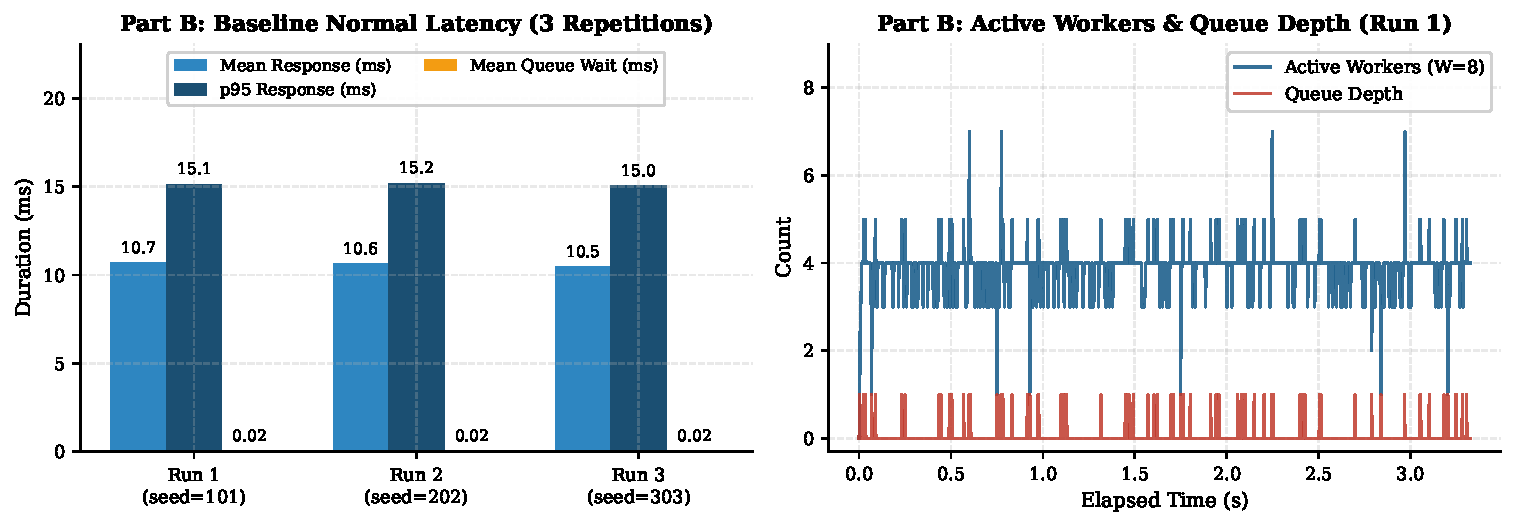
\includegraphics[width=0.95\textwidth]{figures/plot_partB_normal_telemetry.pdf}
    \caption{Part B normal workload telemetry: repeatable latency across 3 seeds (left) and active-worker/queue trace from Run~1 raw JSONL logs (right).}
\end{figure}

% ============================================================================================
% PART C
% ============================================================================================
\newpage
\partheader{Part C --- Automated Correctness and Fault Tests}

\textbf{Commands:} \texttt{STRICT\_INVARIANTS=1 go test -v ./baseline/...} (reproduces baseline failures in \path{data/tests/baseline_strict_fail.log}); \texttt{go test -count=1 -v ./...} and \texttt{go test -count=1 -race -v ./...} (\path{data/tests/*.log}).

\begin{table}[htbp]
\centering
\caption{Automated Test Summary: Strict Baseline vs.\ Improved Service (\texttt{-race} Clean).}
\footnotesize
\begin{tabularx}{\textwidth}{@{} >{\raggedright\arraybackslash}p{2.7cm} >{\raggedright\arraybackslash}X >{\raggedright\arraybackslash}p{3.8cm} >{\raggedright\arraybackslash}p{3.9cm} @{}}
\toprule
\textbf{Test} & \textbf{Fault Injected} & \textbf{Strict Baseline} & \textbf{Improved (\texttt{-race})} \\
\midrule
1. Duplicate-ID & 20--40 duplicate IDs & \textbf{FAIL:} 20 dup outcomes & \textbf{PASS:} 40 blocked, 0 dup \\
2. Cancellation & Cancel at 40\,ms (queued) & \textbf{FAIL:} 229 stranded/lost & \textbf{PASS:} 238 cancelled, 0 lost \\
3. Slow-Worker & 20\% slow (120--150\,ms) & \textbf{FAIL:} 0 T/O, p95=794\,ms & \textbf{PASS:} 26 T/O, $Q_{\max}=32$ \\
4. Failure & Every 10th ID fails & \textbf{PASS:} 135 succ, 15 fail & \textbf{PASS:} 135 succ, 15 fail \\
5. Shutdown & Stop mid-work (80\,ms grace) & \textbf{FAIL:} took 768.7\,ms & \textbf{PASS:} 83.2\,ms, 0 leaks \\
6. Part D Acks & 30\% delay, 30\% dup, 10\% drop & Fails in Part E (477 dups) & \textbf{PASS:} 200/200 succ, 0 dup \\
7. Retry Budget & 50\% drop, budget = 10 & N/A & \textbf{PASS:} capped at 10 retries \\
\bottomrule
\end{tabularx}
\end{table}

\begin{lstlisting}[style=logstyle]
# Strict Baseline Failure Evidence (data/tests/baseline_strict_fail.log)
FAIL: TestDuplicateID      -> I2 VIOLATION (D-01): observed 20 duplicate terminal outcomes
FAIL: TestCancellation     -> I1 VIOLATION (D-02): observed 229 missing/stranded requests
FAIL: TestSlowWorker       -> I6 VIOLATION (D-03): TimedOut=0, MaxQueue=94, p95=794.13ms
FAIL: TestShutdownBounded  -> I4 VIOLATION (D-04): took 768.71ms (> 150ms grace bound)

# Improved Race-Detector Pass (data/tests/improved_race.log): 8/8 PASS, 0 data races (3.673s)
\end{lstlisting}

\textbf{Why \texttt{-race} Is Not Full Correctness:} ThreadSanitizer only detects unsynchronized memory writes along executed paths; it misses logic bugs (D-01), dropped work (D-02), SLA violations (D-03), and deadlocks. Because \texttt{-race} adds heavy overhead (cancel drain rose from 0.81\,ms to 4.66\,ms), race timings are never used as performance benchmarks.

\begin{table}[htbp]
\centering
\caption{Defect Log and Corrective Changes.}
\footnotesize
\begin{tabularx}{\textwidth}{@{} l l >{\raggedright\arraybackslash}X >{\raggedright\arraybackslash}X @{}}
\toprule
\textbf{ID} & \textbf{Inv.} & \textbf{Root Cause} & \textbf{Fix Applied} \\
\midrule
D-01 & I2 & Duplicate IDs re-entered queue and double-recorded. & Intake \texttt{seenIntake} check + \texttt{ResultLedger.CommitOnce}. \\
D-02 & I1 & Workers exited on \texttt{<-stopCh}, stranding queued items. & Workers always drain closed \texttt{workQueue} as \texttt{Cancelled}. \\
D-03 & I6 & Unbounded queue and no per-request timeout. & Per-request \texttt{context.WithTimeout} + bounded queue ($K=64$). \\
D-04 & I4 & Unbounded shutdown drain (768.7\,ms) \& close hazard. & Two-phase \texttt{Shutdown(grace)} with \texttt{intakeMu} admission gate. \\
D-05 & I3 & Logging \texttt{"admitted"} after channel send raced with \texttt{"started"}. & Logged \texttt{"admitted"} strictly \textit{before} channel send under \texttt{intakeMu}. \\
\bottomrule
\end{tabularx}
\end{table}

% ============================================================================================
% PART D
% ============================================================================================
\newpage
\partheader{Part D --- Instructor-Issued Reliability Change}

\textbf{Pre-Coding Record:} \texttt{2026-11-18T15:25:00+05:30} (\path{docs/partD_precoding_record.md}).

\begin{quote}
\itshape ``A downstream acknowledgement may be delayed or repeated. The service must preserve a single terminal result per request while allowing safe recovery after an acknowledgement timeout. Students must specify whether their guarantee is at-most-once processing, at-least-once attempts, or exactly-once recorded outcome; these are not interchangeable.''
\end{quote}

\begin{itemize}
    \item \textbf{Affected Assumptions:} Downstream result collection is no longer synchronous, single-delivery, or append-safe; retries also extend worker holding time unless bounded.
    \item \textbf{Specified Guarantee:} \textbf{Bounded At-Least-Once Acknowledgement Delivery} + \textbf{Exactly-Once Recorded Outcome}. Unlike \textit{at-most-once processing} (which fails fast on transient ack delays), we retry timed-out acks safely; unlike \textit{exactly-once execution}, our guarantee applies strictly to the local \texttt{ResultLedger} unless downstream also deduplicates by \texttt{RequestID}.
    \item \textbf{Design Options:}
    \begin{itemize}
        \item \textit{Option A (Fail-Fast At-Most-Once + Tombstone):} Single ack attempt; timeout commits \texttt{Timeout} and drops late acks. Simple, zero retry traffic, but high false-timeout rate ($\sim$15--20\%).
        \item \textit{Option B (Selected --- Bounded Ack Retry + Idempotent \texttt{ResultLedger}):} Retry timed-out acks (max 3 attempts, 2/4/8\,ms backoff) within a global atomic \texttt{RetryBudget} (25--30\% of $N$). Every ack passes through \texttt{CommitOnce}; late or repeated acks are safely ignored and logged as \texttt{ack\_duplicate\_ignored}.
    \end{itemize}
    \item \textbf{Pre-Coding Prediction:} Baseline will suffer hundreds of duplicate outcomes and false timeouts under \path{configs/ack_faults.json}; Improved will achieve 0 duplicates, 0 accounting violations, high recovery goodput, and $\sim$40--50\,ms p95 (reflecting timeout + retry backoff).
\end{itemize}

% ============================================================================================
% PART E
% ============================================================================================
\clearpage
\partheader{Part E --- Improvement and Controlled Evaluation}

\subhead{E1. Reliability Mechanisms and Evaluation Protocol}
In \path{improved/service.go}, we implemented: (1) \textbf{Idempotent \texttt{ResultLedger.CommitOnce}} (enforces I2; \textit{limit:} in-memory $O(N)$ map needs TTL/DB in daemons), (2) \textbf{Bounded Ack Retry + Global Retry Budget} (caps retry storms; \textit{limit:} permanent outages degrade to \texttt{Timeout}), (3) \textbf{Intake Deduplication}, (4) \textbf{Bounded-Queue Admission Control} ($K=64$; \textit{limit:} rejects excess surge load), and (5) \textbf{Per-Request SLA Timeouts \& Two-Phase Bounded Shutdown}.

\begin{lstlisting}
func (l *ResultLedger) CommitOnce(rec workload.TerminalRecord) bool {
    l.mu.Lock()
    defer l.mu.Unlock()
    if _, exists := l.committed[rec.RequestID]; exists {
        return false // Preserve single immutable terminal outcome (I2)
    }
    l.committed[rec.RequestID] = rec
    l.order = append(l.order, rec)
    return true
}
\end{lstlisting}

\textbf{Metrics \& Denominators:} Both versions ran identical deterministic workloads across 4 conditions $\times$ 3 seeds ($\{101, 202, 303\}$, 24 runs in \path{data/comparison/comparison_raw.csv}; zero missing observations; small variance stems from OS scheduler/timer jitter). We define nearest-rank $\text{p95} = L_{(\lceil 0.95n \rceil)}$ over \textbf{admitted requests only} (excluding $\sim$0.01\,ms fast-rejections so load shedding does not artificially lower latency). Throughput $= N_{\text{unique}}/T_{\text{wall}}$; Goodput $= N_{\text{success}}/T_{\text{wall}}$.

\subhead{E2. Controlled Comparison Results (Baseline vs.\ Improved)}

\begin{table}[htbp]
\centering
\caption{Baseline vs.\ Improved Across All 4 Conditions (Mean $\pm$ SD, 3 Repetitions, $N=1{,}200, W=8$).}
\footnotesize
\setlength{\tabcolsep}{4pt}
\begin{tabularx}{\textwidth}{@{} >{\raggedright\arraybackslash}p{3.6cm} l l >{\raggedright\arraybackslash}X @{}}
\toprule
\textbf{Measure} & \textbf{Baseline} & \textbf{Improved} & \textbf{Key Interpretation} \\
\midrule
\multicolumn{4}{@{}l}{\textbf{Condition 1: Normal Steady-State (\texttt{normal.json}, 450\,req/s, 0\% faults)}} \\
Acct.\ Viol.\ / Dup.\ Out. & $0.0$ / $0.0$ & $0.0$ / $0.0$ & Both satisfy I1/I2 cleanly. \\
Succ.\ / Rej.\ / T/O & 1200 / 0 / 0 & 1200 / 0 / 0 & 100\% success; zero reliability tax. \\
Thru.\ (req/s) & 359.4 & 358.6 & $<0.25\%$ instrumentation overhead. \\
Mean / p95 (ms) & 10.59 / 15.11 & 10.61 / 15.11 & Identical normal latency. \\
Shutdown (ms) / Outst. & 5.19 / 0.0 & 5.40 / 0.0 & Clean empty drain ($\Delta G=0$). \\
\midrule
\multicolumn{4}{@{}l}{\textbf{Condition 2: Overload + Slow Workers (\texttt{overload\_slow.json}, 950\,req/s, 10\% slow 140\,ms, SLA 40\,ms)}} \\
Acct.\ Viol.\ / Dup.\ Out. & $0.0$ / $0.0$ & $0.0$ / $0.0$ & Zero accounting violations. \\
Succ.\ / Rej.\ / T/O & 1200 / 0 / 0 & 958 / 129 / 112 & Sheds 10.8\% surge, aborts 9.4\% slow. \\
Thru.\ / Goodput (req/s) & 326.4 / 326.4 & \textbf{642.8 / 513.3} & Breaks HOL blocking: \textbf{+57.3\% goodput}. \\
Mean / p95 (ms) & 950.6 / 1747.4 & \textbf{101.0 / 142.6} & Bounded queue cuts p95 \textbf{12.3$\times$}. \\
Shutdown (ms) / Outst. & 1902.3 / 0.0 & \textbf{130.2} / 0.0 & Drains \textbf{14.6$\times$ faster}. \\
\midrule
\multicolumn{4}{@{}l}{\textbf{Condition 3: Failure + Mid-Run Shutdown (\texttt{failure\_cancel.json}, 10\% fail, 5\% dup ID, stop 1.1\,s)}} \\
Acct.\ Viol.\ / Dup.\ Out. & 65.7 / 63.7 & \textbf{0.0 / 0.0} & Baseline drops queue + records dups. \\
Succ.\ / Rej.\ / T/O / Fail & 410 / 789 / 0 / 46 & 382 / 746 / 28 / 43 & Improved totals exact 1,200 (vs.\ 1,262). \\
Mean / p95 (ms) & 33.96 / 113.52 & \textbf{13.03 / 50.28} & SLA timeout cuts p95 \textbf{2.3$\times$}. \\
Shutdown (ms) / Outst. & 0.28 / \textbf{2.0} & 13.04 / \textbf{0.0} & Baseline loses queued work; Improved = 0. \\
\midrule
\multicolumn{4}{@{}l}{\textbf{Condition 4: Part D Ack Faults (\texttt{ack\_faults.json}, 15\% delay 45\,ms, 15\% dup ack, 5\% drop, 5\% dup ID)}} \\
Acct.\ Viol.\ / Dup.\ Out. & \textbf{476.7 / 476.7} & \textbf{0.0 / 0.0} & Safely ignores \textbf{415.0} dup/late acks/run. \\
Succ.\ / Rej.\ / T/O / Fail & 1398* / 0 / 230 / 49 & \textbf{1161 / 0 / 0 / 39} & *Baseline inflates Succ $>1200$; Improved recovers all 229.7 ack faults. \\
Thru.\ / Goodput (req/s) & 353.1 / 411.3* & 355.0 / 343.4 & *Misleading Baseline goodput from duplicates. \\
Mean / p95 (ms) & 20.26 / 57.81 & \textbf{16.41 / 41.49} & Bounded retry beats waiting 45\,ms. \\
Shutdown (ms) / Outst. & 83.33 / 0.0 & \textbf{47.61} / 0.0 & Cleaner ack settlement ($\Delta G=0$). \\
\bottomrule
\end{tabularx}
\end{table}

\begin{figure}[htbp]
    \centering
    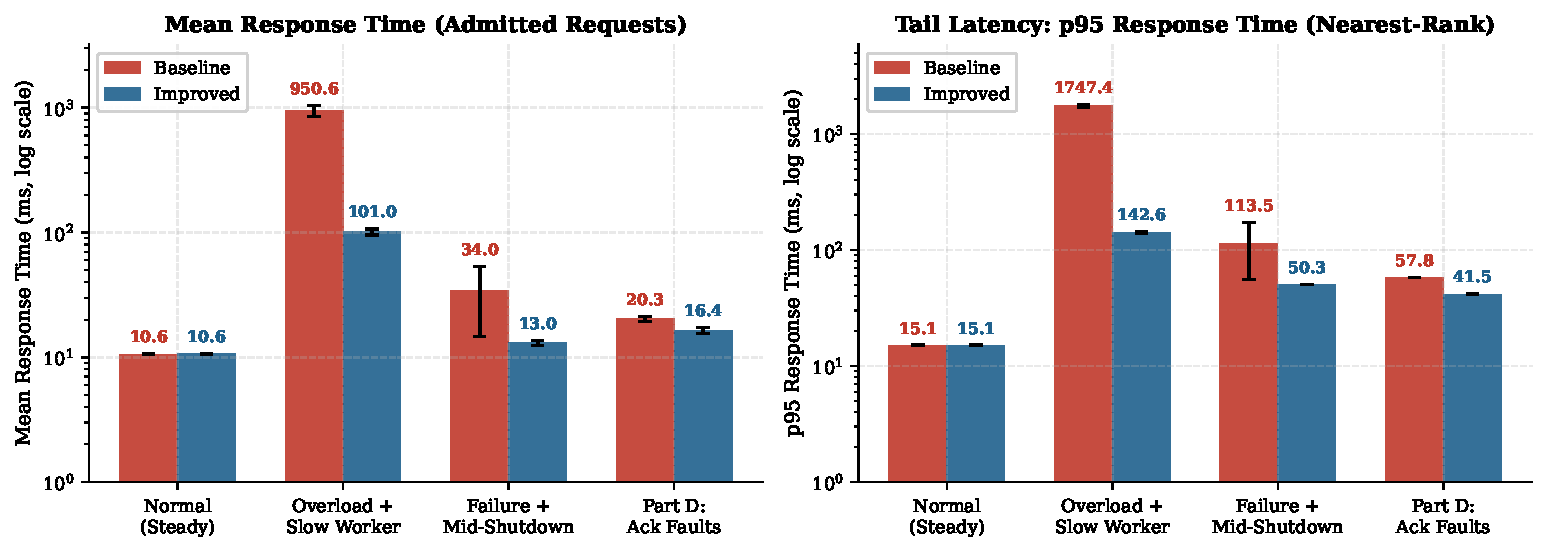
\includegraphics[width=0.95\textwidth]{figures/plot_latency_p95_comparison.pdf}
    \caption{Mean and p95 response times (admitted requests, log scale, mean $\pm$ SD across 3 runs).}
\end{figure}

\newpage
\begin{figure}[htbp]
    \centering
    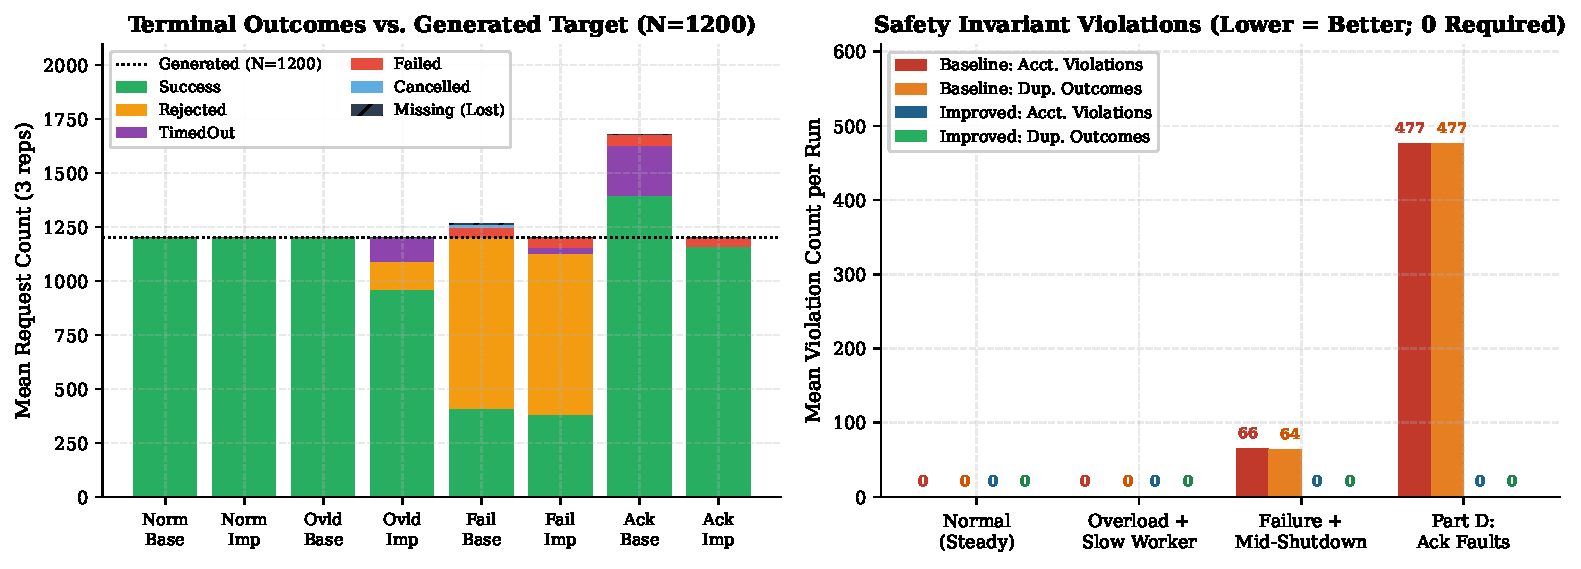
\includegraphics[width=0.95\textwidth]{figures/plot_outcomes_reliability.pdf}
    \caption{Terminal outcome totals vs.\ $N=1{,}200$ (left) and safety invariant violations per run (right).}
\end{figure}

\begin{figure}[htbp]
    \centering
    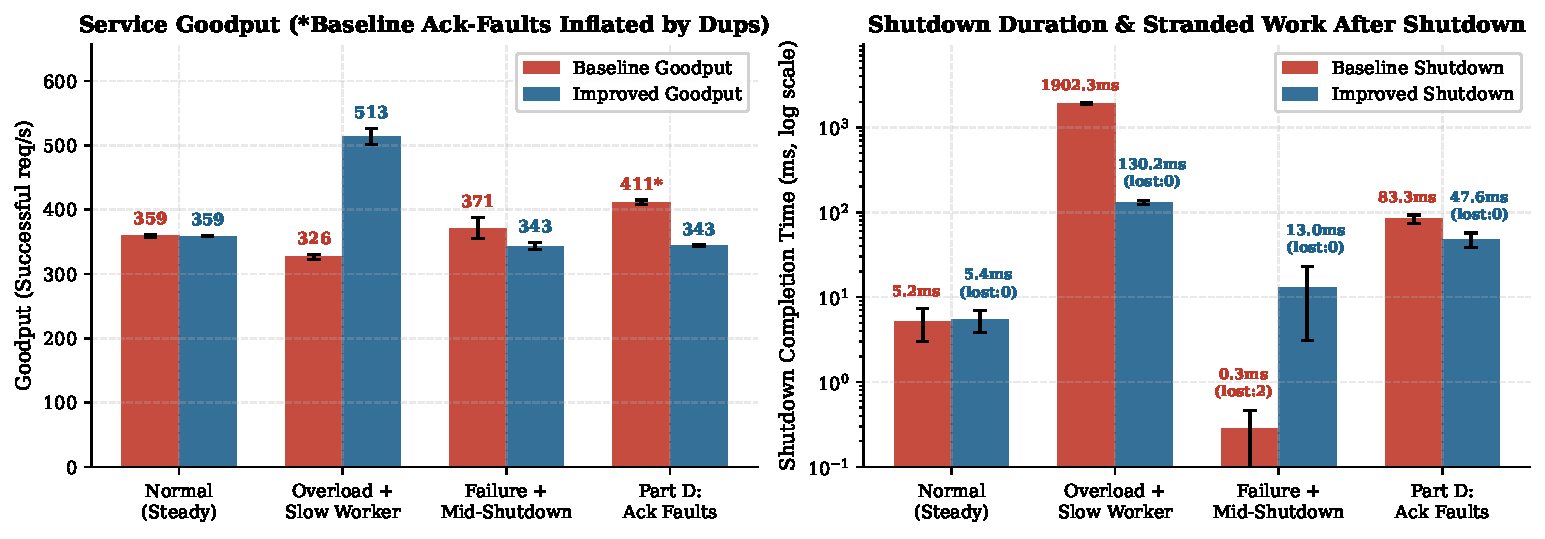
\includegraphics[width=0.95\textwidth]{figures/plot_throughput_shutdown.pdf}
    \caption{Service goodput (left) and shutdown duration with stranded work counts (right).}
\end{figure}

\begin{lstlisting}[style=logstyle]
# Live Part D JSONL trace (data/comparison/improved_ack_faults_run1_events.jsonl)
{"seq":45,"elapsed_ms":33.997,"request_id":9,"event":"ack_duplicate_ignored","reason":"downstream_duplicate_ack_1"}
{"seq":63,"elapsed_ms":44.681,"request_id":2,"event":"ack_retry","reason":"attempt=2 backoff=2ms"}
\end{lstlisting}

% ============================================================================================
% PART F
% ============================================================================================
\clearpage
\partheader{Part F --- Engineering Judgment and Reflection}

\subhead{F1. Reflection Questions}
\begin{enumerate}
    \item \textbf{Hardest invariant:} \textbf{I2} alongside \textbf{I1} under concurrent delayed acks, retries, and shutdown. Without \texttt{CommitOnce}, Baseline logged 476.7 duplicate outcomes/run; Defect D-05 also showed causal ordering fails unless \texttt{"admitted"} is logged before the channel send.
    \item \textbf{Reliability trade-offs:} Under \texttt{overload\_slow}, shedding 10.8\% load and timing out 9.4\% slow tasks cut p95 by 12.3$\times$ and lifted goodput +57.3\%. Under \texttt{ack\_faults}, retry recovery raised p95 from 15.1\,ms to 41.5\,ms to eliminate 229.7 false timeouts ($\sim$440 $\rightarrow$ $\sim$570 LOC).
    \item \textbf{Limits of testing:} Unit tests and \texttt{-race} cover finite in-process schedules only; they cannot rule out \texttt{SIGKILL} crashes, DB deadlocks, TCP resets, GC pauses, or multi-week memory growth.
    \item \textbf{Exactly-once recorded vs.\ execution:} \texttt{ResultLedger} guarantees one immutable local record per \texttt{RequestID}, whereas at-least-once retries can still repeat external side effects unless downstream also deduplicates by \texttt{RequestID}.
    \item \textbf{Pre-deployment test priorities:} (1) Idempotency \& ack-fault tests; (2) Graceful shutdown \& cancellation under \texttt{-race}; (3) Overload + slow-worker SLA tests; (4) Retry-budget exhaustion tests.
    \item \textbf{Additional production evidence:} 24--72\,h soak tests (TTL/LRU eviction), crash/restart tests (\texttt{SIGKILL} + transactional outbox), network fault injection (\texttt{tc-netem}), and canary SLO monitoring.
\end{enumerate}

\subhead{F2. Deployment Recommendation \& Unverified Assumptions}
\textbf{Recommendation:} Deploy \path{improved/service.go} once three controls are added: (1) durable \texttt{ResultLedger}/\texttt{seenIntake} storage (\texttt{UNIQUE(request\_id)} + TTL); (2) end-to-end \texttt{request\_id} idempotency propagation to downstream APIs; and (3) HTTP \texttt{503} + \texttt{Retry-After} shedding with alerts on retry-budget burn and duplicate-ack rates.

\textbf{Unverified Assumptions:} In-process timer simulation (no real TCP/SQL/TLS), volatile memory across restarts, finite batch dedup maps, and transient downstream ack faults.

\textbf{AI Disclosure:} Part~A was completed without generative AI. For Parts~B--F, AI assisted with boilerplate, plotting, and LaTeX formatting; all decisions were verified by the group and \textbf{all results come from live local Go runs}.

\subhead{References \& Contributions}
\textbf{References:} [1] \url{https://go.dev/doc/tutorial/add-a-test}; [2] \url{https://go.dev/doc/articles/race_detector}; [3] \url{https://pkg.go.dev/context}; [4] \url{https://go.dev/blog/pipelines}.

\textbf{Gaurav Acharya [MT26MCS024]:} Part~A analysis/invariants, \path{workload/workload.go}, Part~B baseline, Part~C audit \& D-05 fix, \texttt{ResultLedger}, bounded shutdown. \textbf{Sandeep [MT26MCS032]:} Part~D design/retry-budget spec, ack recovery, admission control, \path{improved/service_test.go}, benchmark/plot scripts, Parts~E--F evaluation.

\end{document}
